\documentclass[11pt]{beamer}
% Packages
\usepackage{beamer-german}


% Title etc.
% Sitzungstitel
\title{Werte \& Wertewandel}
% Veranstaltungstitel
\subtitle{Analyse politischer Unterstützung in der quantitativen Forschungspraxis}
% Datum der Veranstaltung (z.B. 10. Dezember 2021)
\date{\today} 
% Dozent:in
\author{B. Philipp Kleer}
% Affiliation
\institute{Institut für Politikwissenschaft | Justus-Liebig-Universität Gießen}

% selbstgesetzte Größen für Aufzählungen
\setbeamerfont{itemize/enumerate body}{size = \small}
\setbeamerfont{itemize/enumerate subbody}{size = \footnotesize}
\setbeamerfont{itemize/enumerate subsubbody}{size = \scriptsize}

% Datumspaket
\usepackage[german]{isodate}

% Table packages
\usepackage{booktabs}
\usepackage{longtable}

% Quellenverzeichnis zur Sitzung
\addbibresource{lit-s9.bib}

\begin{document}

% Startfolie
\begin{frame}
	\maketitle
\end{frame}


\begin{frame}[t]{Beispiel Tabelle}

% Hier noch Präsentationen und Datum einfügen
	\begin{table}
		\begin{tabular}{m{0.15\textwidth} >{\centering} m{0.1\textwidth} >{\centering} m{0.3\textwidth}  >{\centering\arraybackslash} m{0.3\textwidth}}
			\toprule[2pt]
			\textbf{Datum} & \textbf{Gruppe} & \textbf{Wer?} & \textbf{Feedback}\\
			\midrule
			18.02.2022 & 1 & Wer & ...\\
			\midrule
			18.02.2022 & 2 & Wer & ...\\
			\midrule
			18.02.2022 & 3 & Wer & ...\\
			\midrule
			18.02.2022 & 4 & Wer & ...\\
			\midrule
			18.02.2022 & 5 & Wer & ...\\
			\midrule
			18.02.2022 & 5 & Wer & ...\\
			\bottomrule[2pt]
		\end{tabular}
	\end{table}
% m => horizontal zentriert in Zeile
% p => horizontal top aligned
% b => horizontal bottom aligned
%>{\raggedright} -> rechts aligned
% >{\raggedleft} -> links aligned (default}
% for footnoes: \footnote or footnotemark or footnotetext
\end{frame}

\begin{frame}{Beispiel Itemize}
	\shine{Ziel}: Klären offener Fragen, Erkennen möglicher Fallstricke, Unterstützen bei Projekten

	\begin{itemize}
		\item dazu: aufmerksam Materialien vorher anschauen und aufmerksam zuhören
		\item Feedback wird nicht nur mündlich gegeben, sondern auch schriftlich (Stichpunkte/-sätze reichen, keine formale Form)
			\begin{itemize}
				\item[$\Rightarrow$] Upload in ILIAS
			\end{itemize}
		\item Präsentierende: 3 Tage vor Präsentation Upload der Präsentation und/oder Handout $\Rightarrow$ Donnerstag 23:59h vor Präsentation ist Deadline!
			\begin{itemize}
				\item 10 Minuten Präsentation, 20 Minuten Diskussion	
			\end{itemize}
	\end{itemize}
\end{frame}

\begin{frame}[fragile]{Nummerierte Liste}
Um nummerierte Listen ausgeben zu lassen, bitte \textbf{nolist} nutzen:

\begin{verbatim}
\begin{nolist}
\item erstes item
\item zweites Item
\item drittes Item
\end{nolist}
\end{verbatim}

	\begin{nolist}
		\item erstes item
		\item zweites Item
		\item drittes Item
	\end{nolist}
\end{frame}

\begin{frame}[fragile]{Beispiel Liste mit abc}
Um nummerierte Listen ausgeben zu lassen, bitte \textbf{abclist} nutzen:

\begin{verbatim}
\begin{abclist}
\item erstes item
\item zweites Item
\item drittes Item
\end{abclist}
\end{verbatim}

	\begin{abclist}
		\item erstes item
		\item zweites Item
		\item drittes Item
	\end{abclist}
\end{frame}


\begin{frame}{Beispiel Zitation \& Itemize}
	\begin{itemize}
		\item \cite{Welzel2013}: 
		\item \cite{Inglehart2010}: 
		\item \cite{Scherer2020}:
		\item \cite{Welzel2009}:
	\end{itemize}
\end{frame}


\begin{frame}{Beispiel Grafik einfügen}
	\begin{figure}[ht]
		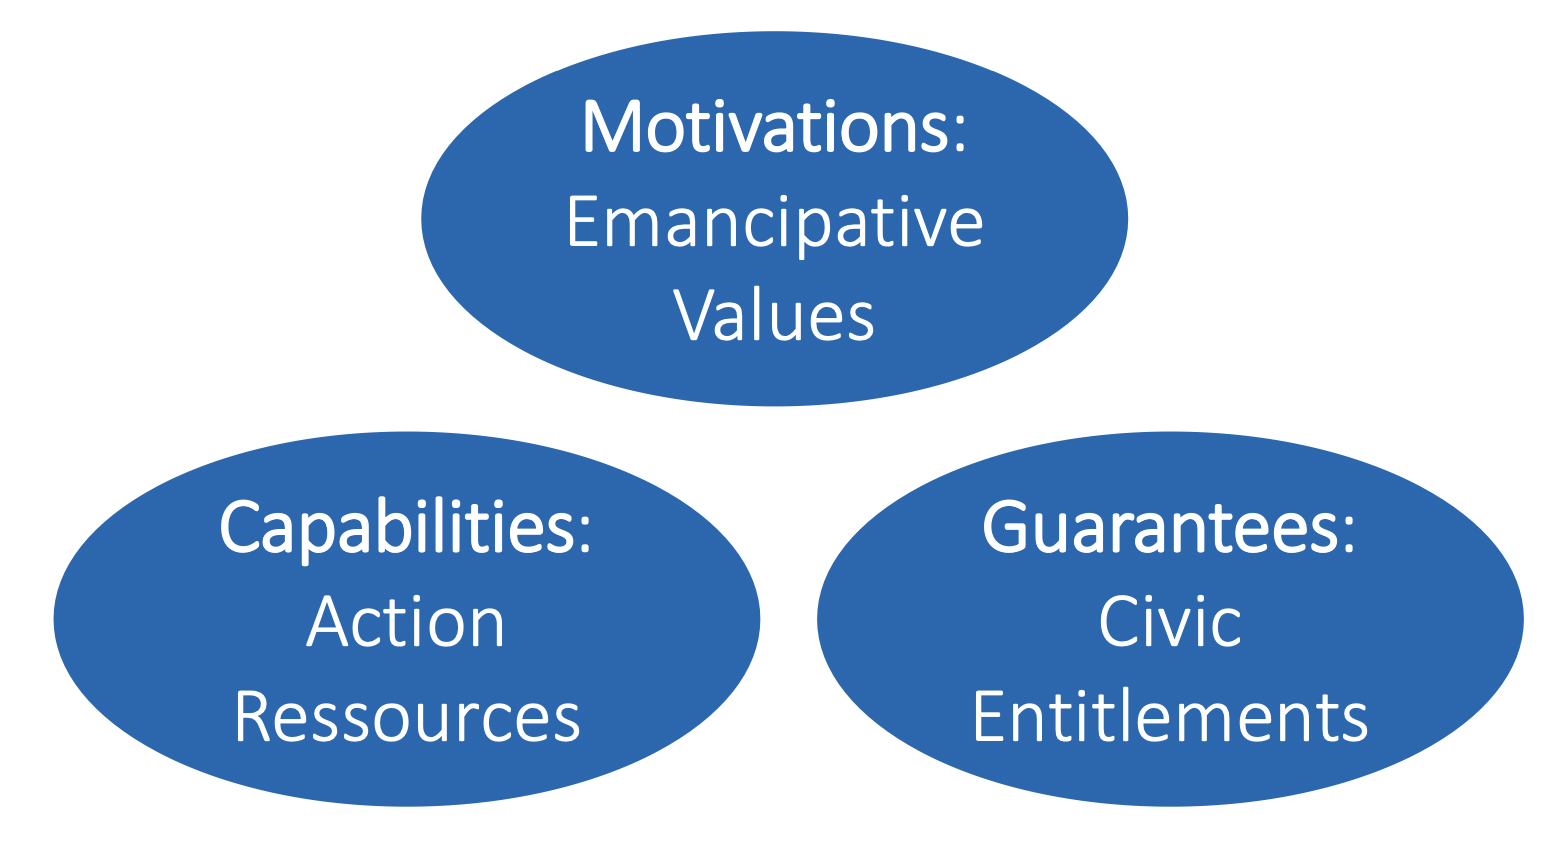
\includegraphics[width=\textwidth]{pics/s9-1.png}
		\caption{\textbf{Theoretischer Überblick}}
	\end{figure}
\end{frame}

\begin{frame}{Beispiel Spaltenlayout}
	\begin{columns}
		\begin{column}{0.3\textwidth}
			\begin{figure}[ht]
				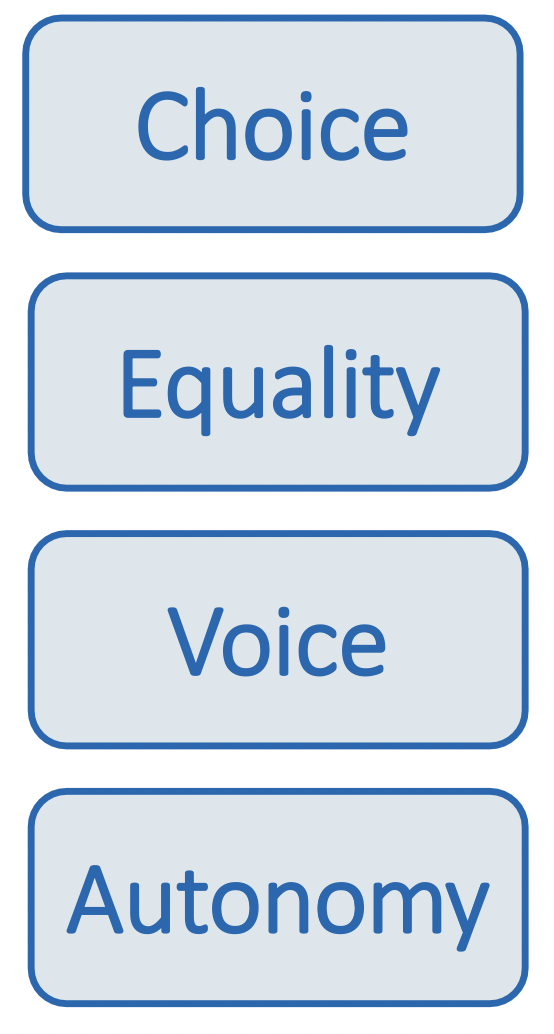
\includegraphics[width=\textwidth]{pics/s9-2.png}
			\end{figure}
		\end{column}
		\begin{column}{0.7\textwidth}
			\begin{itemize}
				\item Tolerance of Abortion, Divorce and Homosexuality
				\item[]
				\item Women‘s equality (Politic, Education, Job)
				\item[]
				\item Priority more to say (local/national)
				\item Freedom of Speech
				\item Independence a desired quality
				\item Obedience not a desired quality
				\item Imagination a desired quality
			\end{itemize}
		\end{column}
	\end{columns}
\end{frame}


% Setzen Schriftgröße für Literatur-Slides (kleiner, damit es nicht so viele sind
\renewcommand*{\bibfont}{\scriptsize}

% automatisch alle Quellen, die in bib sind (wenn nicht gewünscht einfach \nocite{*} auskommentieren
% allowframebreaks macht automatisch mehrere slides, wenn es nicht auf eine passt.
\begin{frame}[allowframebreaks]{Literatur}
	\nocite{*}
	\printbibliography[heading = none]
\end{frame}

% Abschiedsslide
\section{Wir sehen uns in zwei Wochen!}
%\section{Mittagspause! \\ Wir treffen uns um 12:30 Uhr wieder.}

\end{document}
